\documentclass[11pt]{article}
\usepackage{geometry}                % See geometry.pdf to learn the layout options. There are lots.
\geometry{letterpaper}
\pagestyle{empty}                   % ... or a4paper or a5paper or ... 
\oddsidemargin 0in
\evensidemargin 0in
\textwidth 6.5in
%\headheight 0in
\topmargin 0in
\textheight 8.1in
%\footheight 0in 
%\geometry{landscape}                % Activate for for rotated page geometry
%\usepackage[parfill]{parskip}    % Activate to begin paragraphs with an empty line rather than an indent
\usepackage{graphicx}
\usepackage{amssymb}
\usepackage{epstopdf}
\DeclareGraphicsRule{.tif}{png}{.png}{`convert #1 `dirname #1`/`basename #1 .tif`.png}

\title{Midterm exam: BIOS 26210}
\author{}
\date{}                                           % Activate to display a given date or no date

\begin{document}
\maketitle
%\section{}
%\subsection{}
\begin{enumerate}

\item The following discrete time model may be used to model density-limited population growth, where $t$ is the time, expressed in number of generations, and $N$ is the population size:
 $$N_{t+1} = r \frac{N_t}{1+N_t}$$
\begin{enumerate}

\item Here $N$ is a dimensionless population size. Find the dimensions of $r$, and explain its biological significance.

\item Find the fixed point(s) (equilibria) of the system, and describe their biological meaning.

\item Determine the condition of stability of the fixed points in terms of the parameter $r$.

\item Find any bifurcations that depend on $r$, and classify them.

\item Describe the long-term behavior of the population for $r=2$, and sketch its progress over time, starting with a reasonable initial value.
\end{enumerate}


\item The Gompertz model describes the growth of cancer cells in a tumor, where $x$ is the number of cells and $t$ is time. It is a modified linear growth model with a time-dependent coefficient:
$$ \dot x = k e^{- at} x$$
\begin{enumerate}
\item Assume the dimensions of $k$ are the same as in a linear population model (inverse time). What are the dimensions of $a$, and what is its significance? 
\item Find the analytical solution by separating the variables ($x$ and $t$) and integrating both sides.
\item Use the initial condition $x(0) = x_0$ to solve for the integration constant.
\item Based on this solution, what is the long-term behavior of the model? Does the future tumor size depend on the initial value $x_0$?
\end{enumerate}


\begin{center}
\Large{(OVER)}
\end{center}
\newpage
\item Consider the following function: $ f(x) = -0.3x(x+2)(x-4)$, with the graph shown in the figure below.
\begin{enumerate}
\item For the ODE $\dot x = f(x)$, find the fixed points and their stability, based on the graph of $f(x)$. 
\item Suppose that $x(0) = 1$. Sketch the time course of the solution $x(t)$ on a separate graph. 
\item Add a constant parameter to the system: $\dot x = -0.3x(x+2)(x-4)+ r$. Without performing any calculations, describe the types of bifurcations that occur as $r$ varies, and predict the approximate bifurcation values of $r$.
\item Now consider the discrete time system $X_{t+1} = f(X_t)$. Based on the graph, indicate the approximate values of the fixed points, and predict their stability. 
\item Find the fixed points analytically and perform linear stability analysis for them. Explain how it relates to the graphical analysis.
\item On a separate plot, sketch the cobweb plot for the solution starting with $X_0 = -1$ for a few iterations. What is the long-term behavior of the solution?

\end{enumerate}

\begin{figure}[htbp] %  figure placement: here, top, bottom, or page
   \centering
   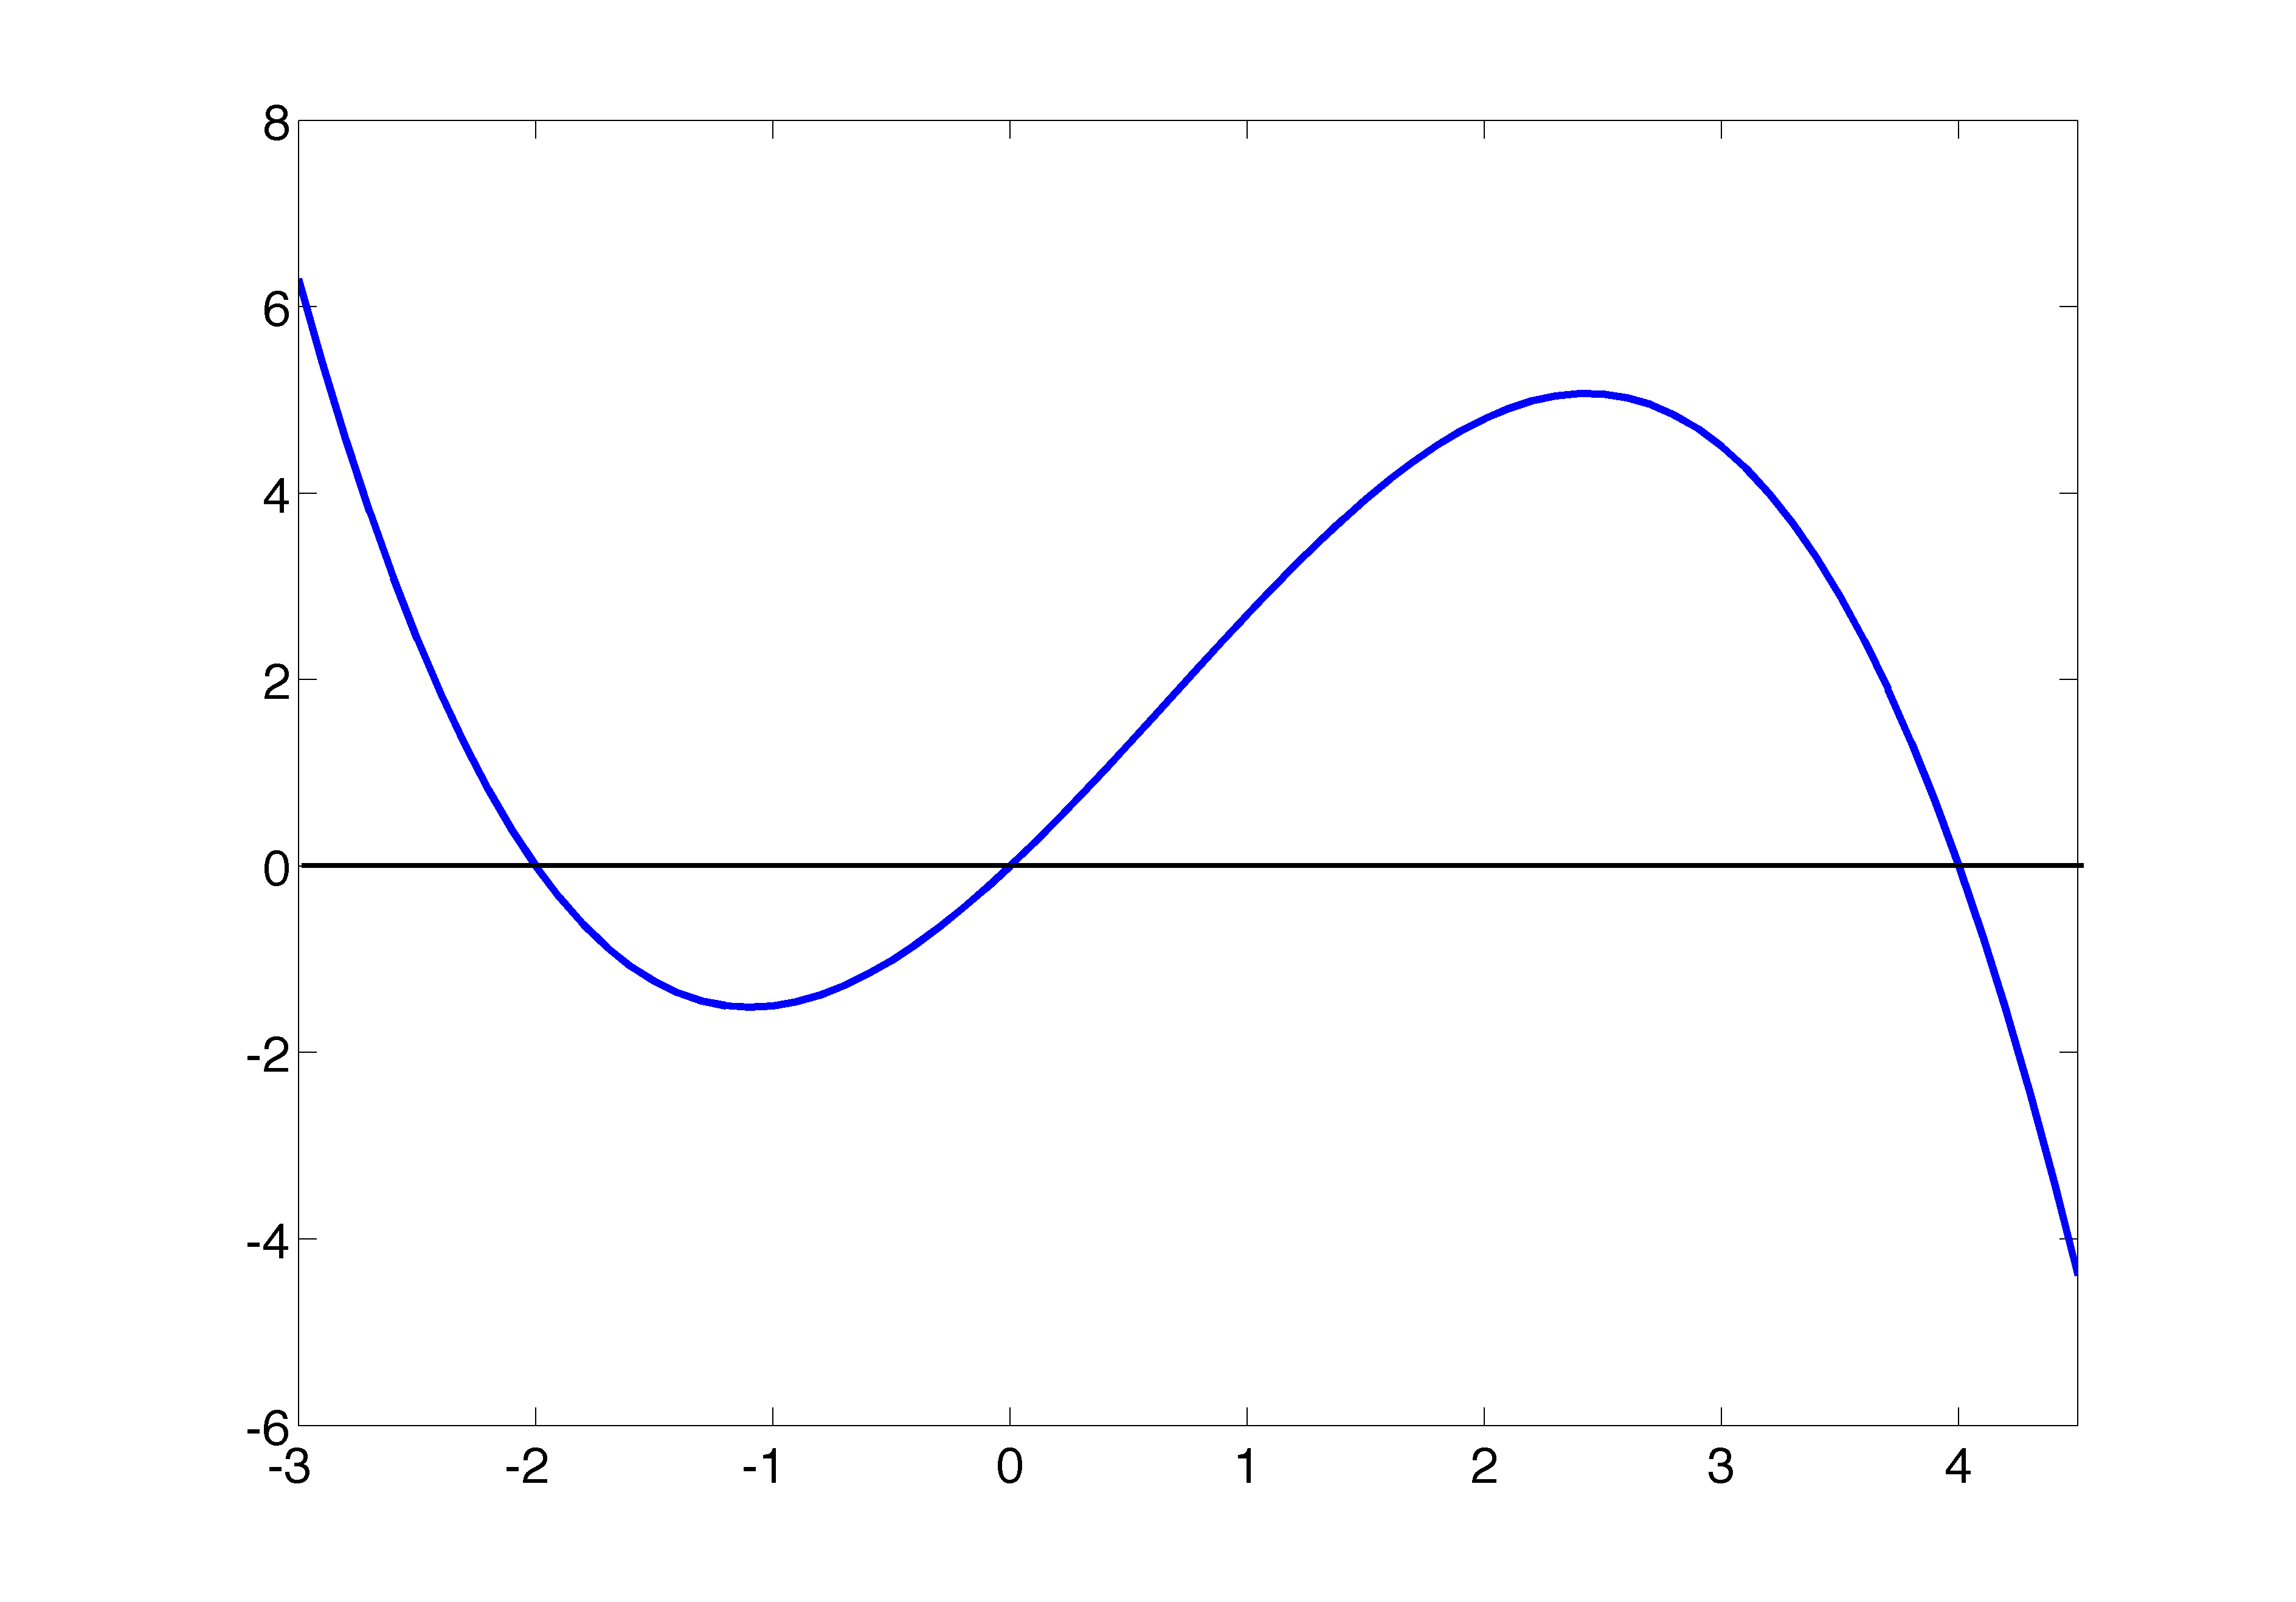
\includegraphics[width=5in]{mid_func.png} 
   \caption{Plot of  $f(x)$ }
   \label{fig:example}
\end{figure}




\end{enumerate}
\end{document}  